% Options for packages loaded elsewhere
\PassOptionsToPackage{unicode}{hyperref}
\PassOptionsToPackage{hyphens}{url}
%
\documentclass[
  ignorenonframetext,
]{beamer}
\usepackage{pgfpages}
\setbeamertemplate{caption}[numbered]
\setbeamertemplate{caption label separator}{: }
\setbeamercolor{caption name}{fg=normal text.fg}
\beamertemplatenavigationsymbolsempty
% Prevent slide breaks in the middle of a paragraph
\widowpenalties 1 10000
\raggedbottom
\setbeamertemplate{part page}{
  \centering
  \begin{beamercolorbox}[sep=16pt,center]{part title}
    \usebeamerfont{part title}\insertpart\par
  \end{beamercolorbox}
}
\setbeamertemplate{section page}{
  \centering
  \begin{beamercolorbox}[sep=12pt,center]{part title}
    \usebeamerfont{section title}\insertsection\par
  \end{beamercolorbox}
}
\setbeamertemplate{subsection page}{
  \centering
  \begin{beamercolorbox}[sep=8pt,center]{part title}
    \usebeamerfont{subsection title}\insertsubsection\par
  \end{beamercolorbox}
}
\AtBeginPart{
  \frame{\partpage}
}
\AtBeginSection{
  \ifbibliography
  \else
    \frame{\sectionpage}
  \fi
}
\AtBeginSubsection{
  \frame{\subsectionpage}
}
\usepackage{amsmath,amssymb}
\usepackage{lmodern}
\usepackage{iftex}
\ifPDFTeX
  \usepackage[T1]{fontenc}
  \usepackage[utf8]{inputenc}
  \usepackage{textcomp} % provide euro and other symbols
\else % if luatex or xetex
  \usepackage{unicode-math}
  \defaultfontfeatures{Scale=MatchLowercase}
  \defaultfontfeatures[\rmfamily]{Ligatures=TeX,Scale=1}
\fi
% Use upquote if available, for straight quotes in verbatim environments
\IfFileExists{upquote.sty}{\usepackage{upquote}}{}
\IfFileExists{microtype.sty}{% use microtype if available
  \usepackage[]{microtype}
  \UseMicrotypeSet[protrusion]{basicmath} % disable protrusion for tt fonts
}{}
\makeatletter
\@ifundefined{KOMAClassName}{% if non-KOMA class
  \IfFileExists{parskip.sty}{%
    \usepackage{parskip}
  }{% else
    \setlength{\parindent}{0pt}
    \setlength{\parskip}{6pt plus 2pt minus 1pt}}
}{% if KOMA class
  \KOMAoptions{parskip=half}}
\makeatother
\usepackage{xcolor}
\newif\ifbibliography
\usepackage{longtable,booktabs,array}
\usepackage{calc} % for calculating minipage widths
\usepackage{caption}
% Make caption package work with longtable
\makeatletter
\def\fnum@table{\tablename~\thetable}
\makeatother
\usepackage{graphicx}
\makeatletter
\def\maxwidth{\ifdim\Gin@nat@width>\linewidth\linewidth\else\Gin@nat@width\fi}
\def\maxheight{\ifdim\Gin@nat@height>\textheight\textheight\else\Gin@nat@height\fi}
\makeatother
% Scale images if necessary, so that they will not overflow the page
% margins by default, and it is still possible to overwrite the defaults
% using explicit options in \includegraphics[width, height, ...]{}
\setkeys{Gin}{width=\maxwidth,height=\maxheight,keepaspectratio}
% Set default figure placement to htbp
\makeatletter
\def\fps@figure{htbp}
\makeatother
\setlength{\emergencystretch}{3em} % prevent overfull lines
\providecommand{\tightlist}{%
  \setlength{\itemsep}{0pt}\setlength{\parskip}{0pt}}
\setcounter{secnumdepth}{-\maxdimen} % remove section numbering
\ifLuaTeX
  \usepackage{selnolig}  % disable illegal ligatures
\fi
\IfFileExists{bookmark.sty}{\usepackage{bookmark}}{\usepackage{hyperref}}
\IfFileExists{xurl.sty}{\usepackage{xurl}}{} % add URL line breaks if available
\urlstyle{same} % disable monospaced font for URLs
\hypersetup{
  pdftitle={The evolution of SOC modeling},
  pdfauthor={Lorenzo Menichetti},
  hidelinks,
  pdfcreator={LaTeX via pandoc}}

\title{The evolution of SOC modeling}
\author{Lorenzo Menichetti}
\date{2023-05-19}

\begin{document}
\frame{\titlepage}

\begin{frame}{Soil organic matter gets interesting (1804)}
\protect\hypertarget{soil-organic-matter-gets-interesting-1804}{}
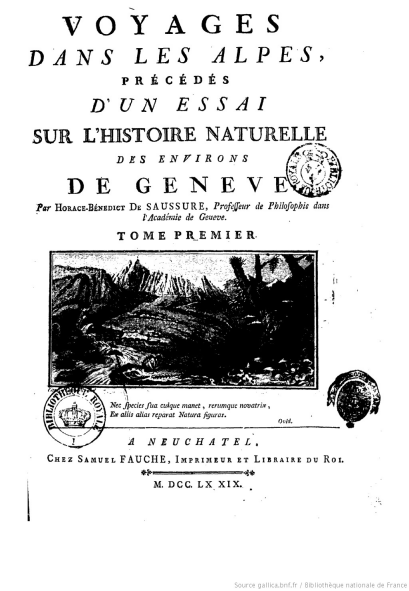
\includegraphics[width=\textwidth,height=0.5\textheight]{Saussure.png}

Some systematic observations about SOM:

\begin{enumerate}
\tightlist
\item
  since no continuous accumulation of SOM occurs even with continuous
  organic inputs, some of these inputs must be destroyed,
\item
  the amount which is destroyed must, to a certain extent, be
  proportional to the absolute existing amount,
\item
  limits to SOM accretion must vary depending on climate, nature of
  mother bedrock, vegetation, cropping system and fertility of the land,
\item
  even if all conditions are favorable to SOM accumulation, there must
  be a maximum for the thickness of the humus layer beyond which
  destructive causes equal productive ones.
\end{enumerate}
\end{frame}

\begin{frame}{Soil organic matter gets attention (1938)}
\protect\hypertarget{soil-organic-matter-gets-attention-1938}{}
A more structured approach to understand its nature initiated during
past century:

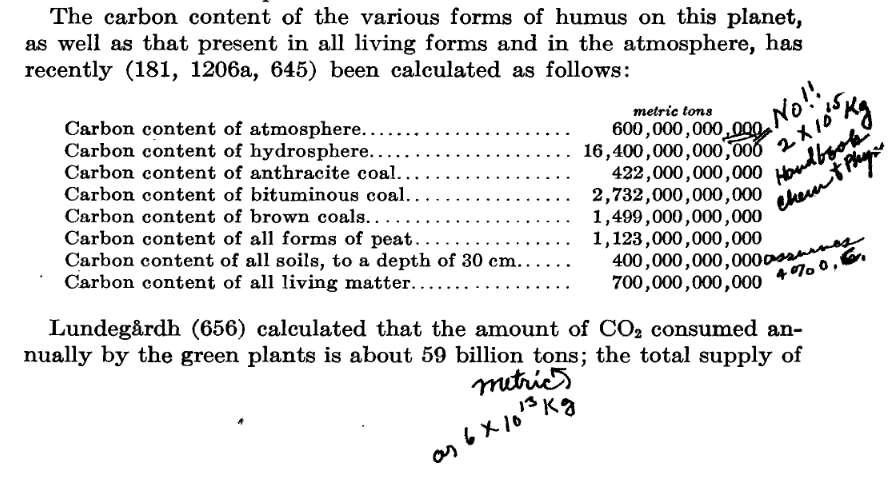
\includegraphics[width=0.7\textwidth,height=\textheight]{waksman_1938.png}

\emph{Waksman, S.A., 1938. Humus. Origin, Chemical Composition and
Importance in Nature, second ed.~revised. Williams and Wilkins,
Baltimore, p.~526}
\end{frame}

\begin{frame}{The Beginning of the conventional SOC decay theory (1945)}
\protect\hypertarget{the-beginning-of-the-conventional-soc-decay-theory-1945}{}
Hénin and Dupuis are probably the first to conceptualize a SOC (\(C_s\))
decay model: \[
\frac{dC_s}{dt} = h \cdot C_i - k \cdot C_s
\] In their formulation, the inputs to the SOC are defined by the C
inputs \(C_i\) times a humification constant \(h\).

\includegraphics{Presentation_files/figure-beamer/unnamed-chunk-1-1.png}
\end{frame}

\begin{frame}{The Beginning of the conventional SOC decay theory (1963)}
\protect\hypertarget{the-beginning-of-the-conventional-soc-decay-theory-1963}{}
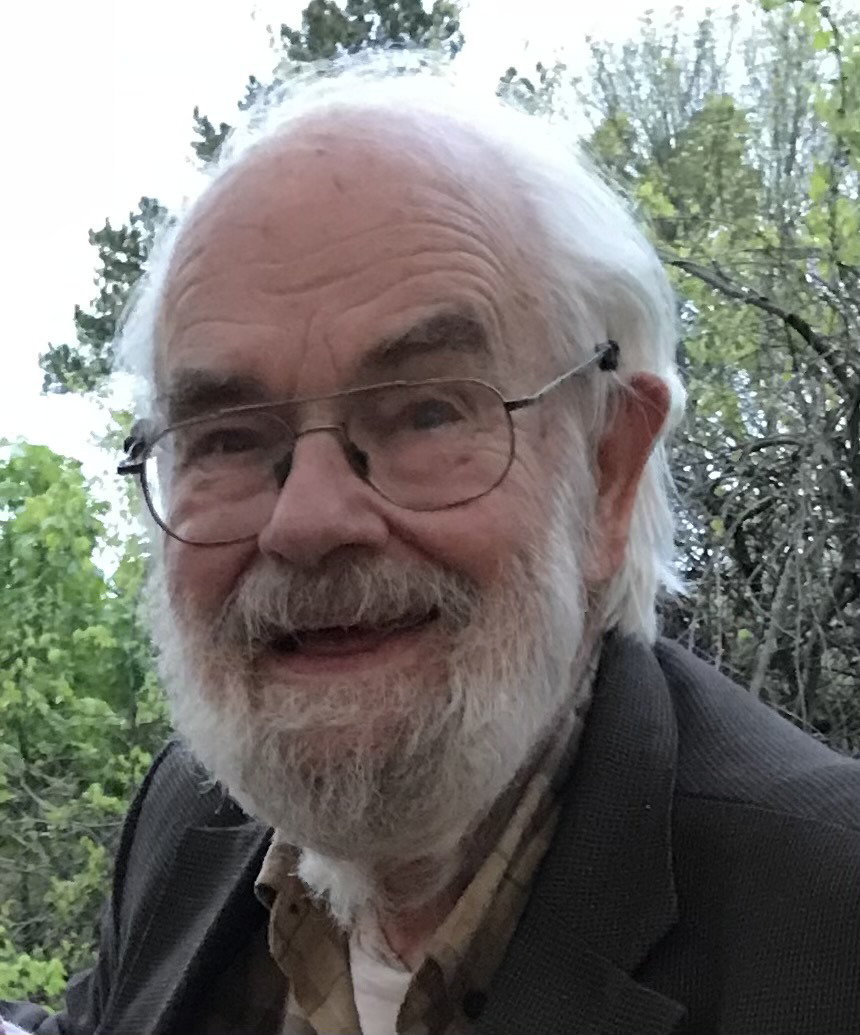
\includegraphics[width=0.5\textwidth,height=\textheight]{Olson.jpg}

Jerry Olson stated in the incipit of his SOC modeling paper: \emph{``The
net rate of change in energy or material stored in an ecological system
or its parts equals the \textbf{rate of income} minus the \textbf{rate
of loss}.''}

\includegraphics{Presentation_files/figure-beamer/unnamed-chunk-2-1.png}

And described it mathematically with a linear differential equation very
similar to Hénin and Dupuis model: \[
\frac{dC_s}{dt} = I - k \cdot C_s
\] Compared to Hénin and Dupuis, the term \(I\) substitutes
\(h \cdot C_i\), but since \(h\) is anyway a latent variable the two
models are virtually the same. Such equation is still the basis for most
SOC models available around.
\end{frame}

\begin{frame}{Differences between Olson and Hénin \& Dupuis}
\protect\hypertarget{differences-between-olson-and-huxe9nin-dupuis}{}
While Olson's model is actually a single pool model, Hénin \& Dupuis
define the input flux to the soil as a fraction of the total C input
\(C_i\), which can describe the litter. When considering the implicit
fluxes from the system (respiration), in order to close the mass
balance, we need to account also for the respiration from the litter:

\includegraphics{Presentation_files/figure-beamer/unnamed-chunk-3-1.png}
\end{frame}

\begin{frame}{Many many many many SOC models}
\protect\hypertarget{many-many-many-many-soc-models}{}
A \textbf{(for sure incomplete)} list of the major (only linear ones,
we'll come to this later) SOC models over time:

\includegraphics{Presentation_files/figure-beamer/unnamed-chunk-4-1.png}
\end{frame}

\begin{frame}{The Golden Era: RothC (1977)}
\protect\hypertarget{the-golden-era-rothc-1977}{}
\end{frame}

\begin{frame}{The Golden Era: Century (1987)}
\protect\hypertarget{the-golden-era-century-1987}{}
\end{frame}

\begin{frame}{An interesting outlier: Q}
\protect\hypertarget{an-interesting-outlier-q}{}
\end{frame}

\begin{frame}{The problem of model initialization}
\protect\hypertarget{the-problem-of-model-initialization}{}
\end{frame}

\begin{frame}{The dream of ``data-based'' initialization: Yasso,
Zimmerman, etc\ldots{}}
\protect\hypertarget{the-dream-of-data-based-initialization-yasso-zimmerman-etc}{}
\end{frame}

\begin{frame}{Things get complicated}
\protect\hypertarget{things-get-complicated}{}
Soil C models are required to represent more things than just the
aerobic C decomposition process.\\
In the most recent decades we can observe a very large amount of models
being published that are based on many different processes and integrate
many components (es. ECOSSE, ORCHIDEE, DayCent).
\end{frame}

\begin{frame}{Representing reality?}
\protect\hypertarget{representing-reality}{}
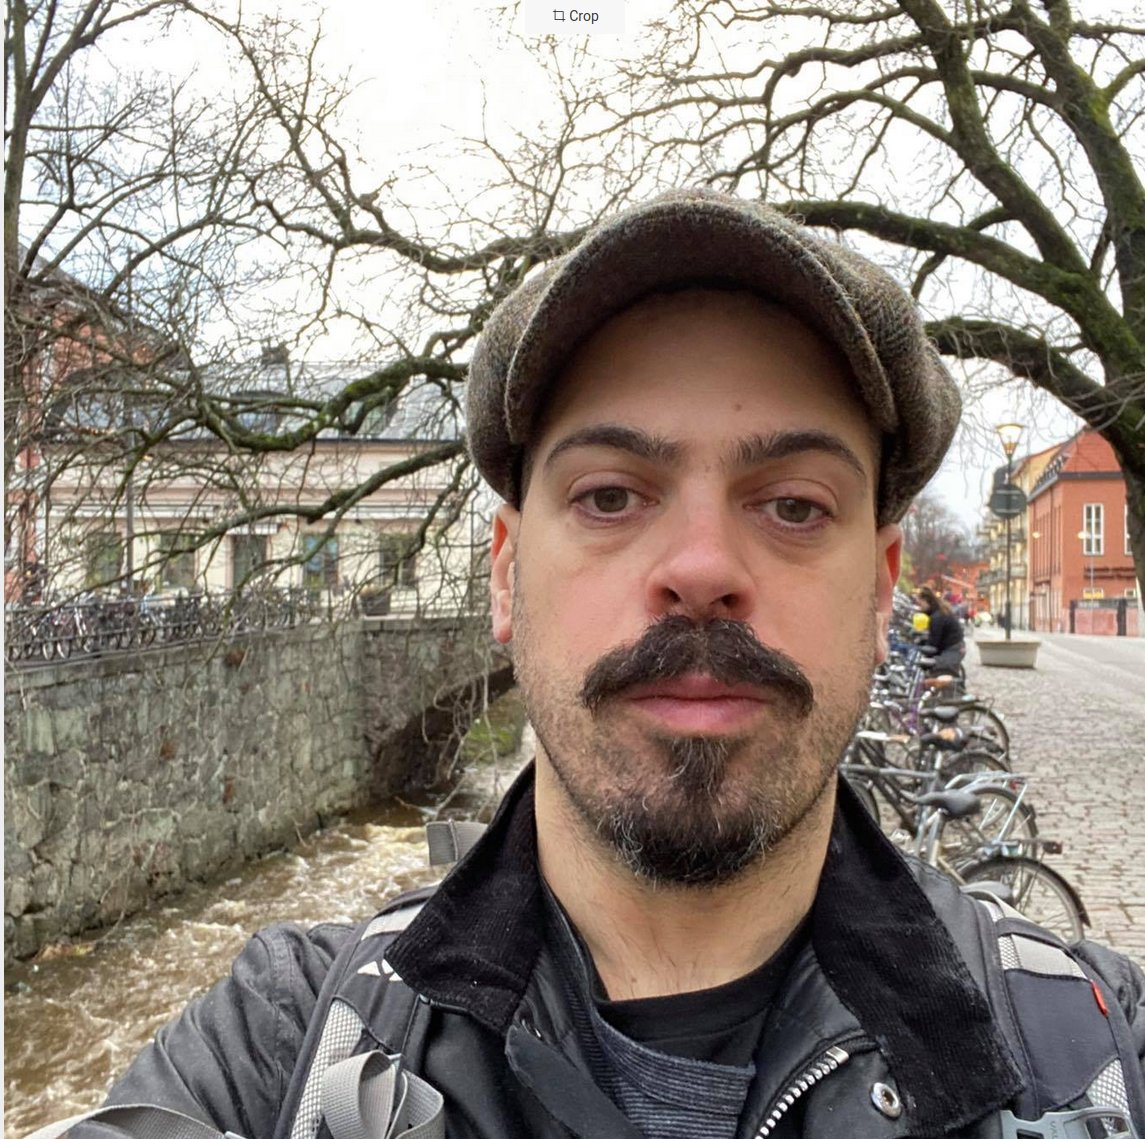
\includegraphics[width=\textwidth,height=3.64583in]{me.jpg} 316 kB

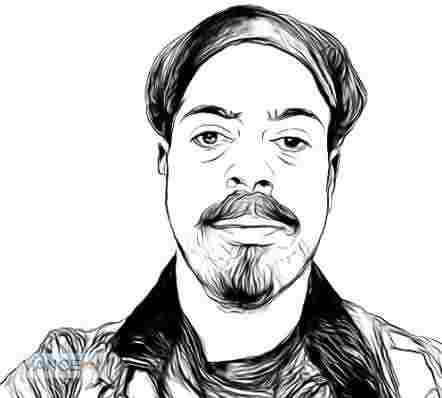
\includegraphics[width=\textwidth,height=3.64583in]{me_model.jpg} 11 kB
\end{frame}

\begin{frame}{One possible tree of SOC models concepts}
\protect\hypertarget{one-possible-tree-of-soc-models-concepts}{}
\includegraphics{Presentation_files/figure-beamer/unnamed-chunk-5-1.png}
\end{frame}

\begin{frame}{The basic SOM model choices}
\protect\hypertarget{the-basic-som-model-choices}{}
\begin{itemize}
\tightlist
\item
  Do we assume some ``inert'' SOM?
\item
  How many different C pools do we represent?
\item
  Do we represent mass feedbacks?
\item
  Is it fine to use ordinary differential equations, or do we need PDE?
\end{itemize}

Each of these choices will bring implications in the extrapolation we
can do with the model, some quite dramatic.
\end{frame}

\begin{frame}{The advantages of minimalism: easily solved steady states}
\protect\hypertarget{the-advantages-of-minimalism-easily-solved-steady-states}{}
No system will accumulate or lose C indefinitely. The rates will always
tend to zero.\\
When the rate of SOC variation is zero, the system is in
\textbf{equilibrium}, and inputs equal outputs. For example a land use
change from a relatively rich environment (a forest) to an environment
with less C inputs (agriculture). SOC will decrease over time until it
reaches the new equilibrium:

\includegraphics[width=0.5\linewidth]{Presentation_files/figure-beamer/unnamed-chunk-6-1}
\end{frame}

\begin{frame}{The advantages of minimalism: easily solved steady states}
\protect\hypertarget{the-advantages-of-minimalism-easily-solved-steady-states-1}{}
The steady states are, by definition, where the rate of variation
\(\frac{dC}{dt}=0\). For a single pool model (Olson) this becomes easily
solved. The steady state means that for a certain amount of C \(C_{ss}\)
the variation is zero: \(0 = I - k \cdot C_{ss}\), which means
\(k \cdot C_{ss} = I\) and therefore \(C_{ss}=\frac{I}{k}\).

A slightly more complicated model, like the two pool (Y and O) ICBM, has
still relatively simple analyitcal solution: \[
Y_{ss}=\frac{I}{k_y}\\
O_{ss}=\epsilon\cdot\frac{I}{k_o}
\] Any linear model, with an arbitrary number of pools, has an
analytical solution. But having it so short and easily manageable can
sometimes be useful.
\end{frame}

\begin{frame}{The advantages of more pools: long-term accuracy}
\protect\hypertarget{the-advantages-of-more-pools-long-term-accuracy}{}
\end{frame}

\begin{frame}{The cyclical discussion: ``breaking'' SOC decomposition
paradigm?}
\protect\hypertarget{the-cyclical-discussion-breaking-soc-decomposition-paradigm}{}
\end{frame}

\begin{frame}{Representing reality: the view of experimentalists}
\protect\hypertarget{representing-reality-the-view-of-experimentalists}{}
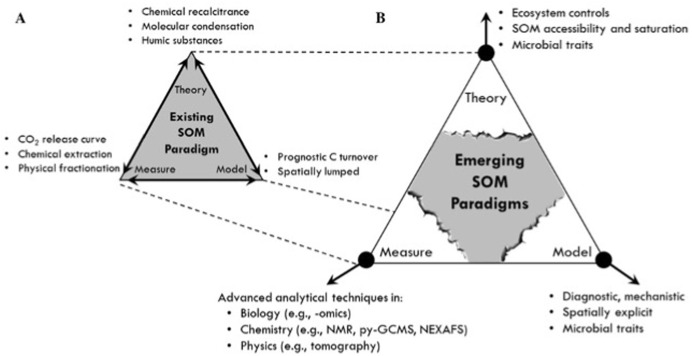
\includegraphics[width=0.7\textwidth,height=\textheight]{Schimel.jpg}
\emph{Schimel, Joshua. ``Modeling Ecosystem-Scale Carbon Dynamics in
Soil: The Microbial Dimension.'' Soil Biology and Biochemistry 178
(March 2023)}
\end{frame}

\begin{frame}{Representing reality: the view of experimentalists}
\protect\hypertarget{representing-reality-the-view-of-experimentalists-1}{}
We know that SOC decomposition is process mediated by microbes, their
growth and by their exoenzymes production, so representing these
processes will produce more accurate models.

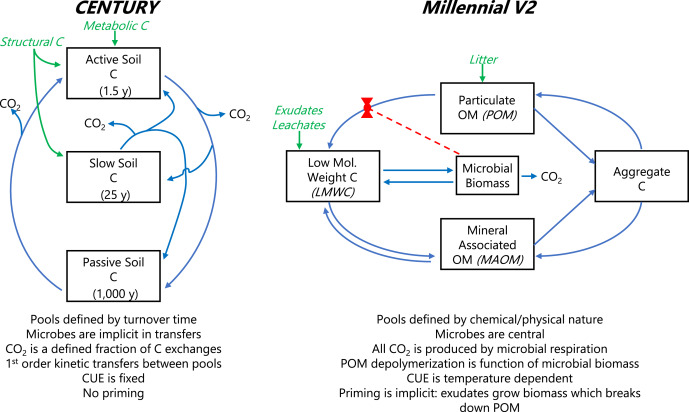
\includegraphics[width=0.55\textwidth,height=\textheight]{Schimel2.jpg}
\emph{Schimel, Joshua. ``Modeling Ecosystem-Scale Carbon Dynamics in
Soil: The Microbial Dimension.'' Soil Biology and Biochemistry 178
(March 2023)}
\end{frame}

\begin{frame}{The cyclical discussion: is more realistic more better?}
\protect\hypertarget{the-cyclical-discussion-is-more-realistic-more-better}{}
Making decomposition controlled by enzymes/microbes means making the
model nonlinear, moving from ordinary differential equations to partial
differential equations.

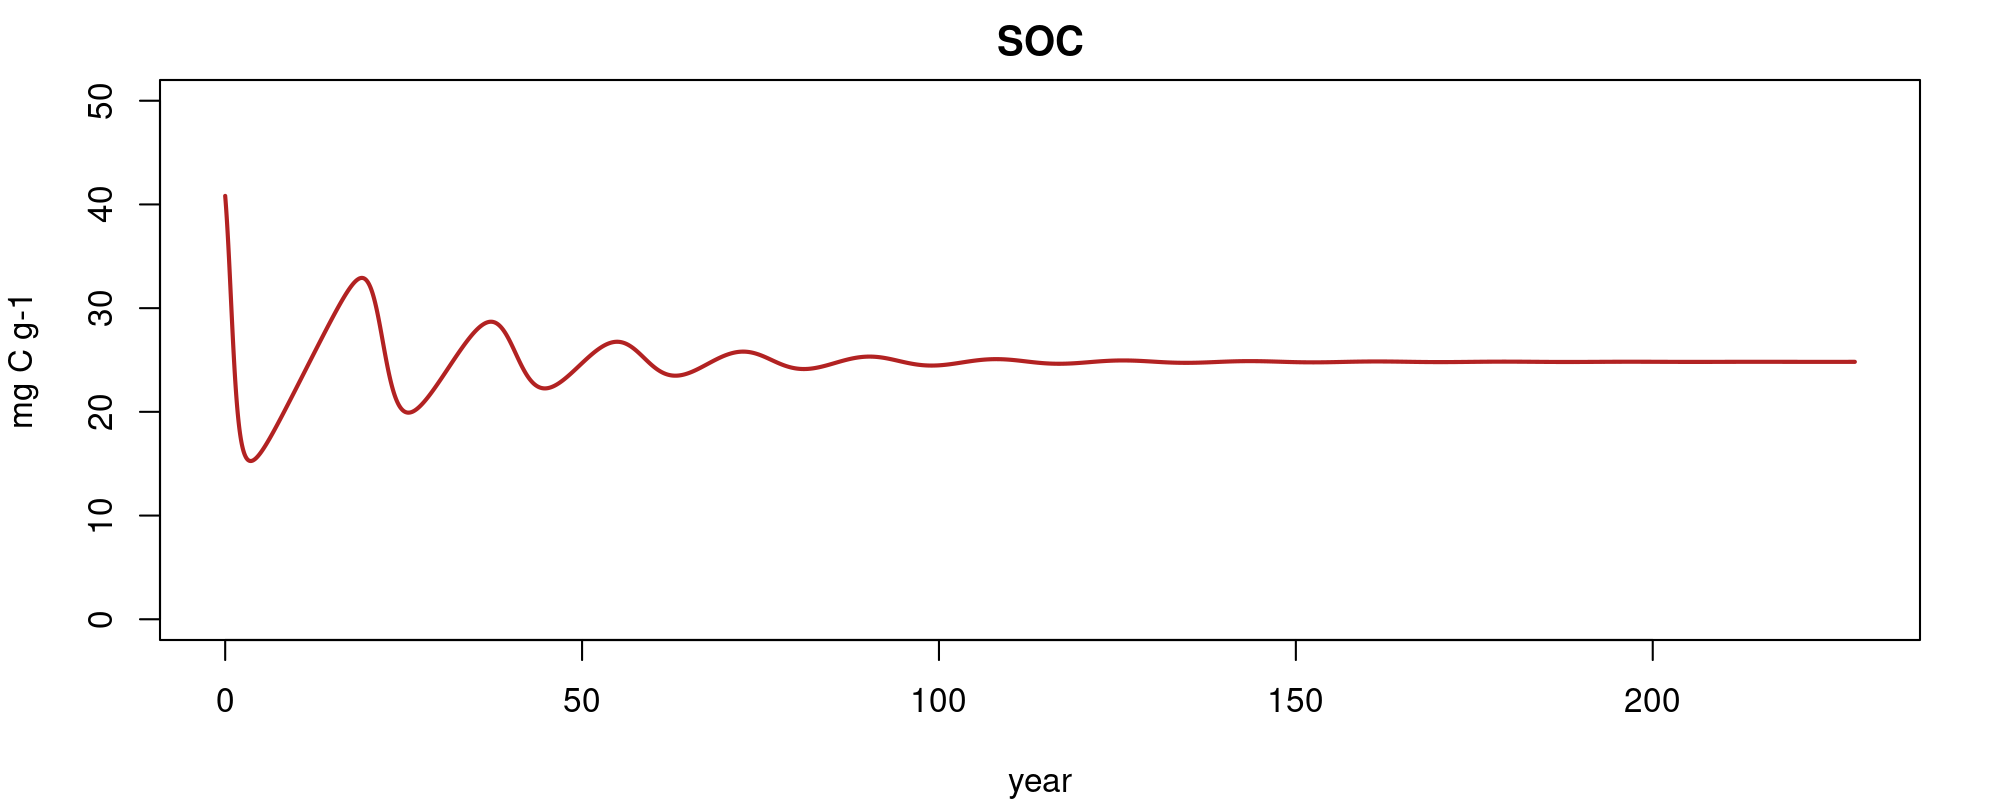
\includegraphics[width=0.6\textwidth,height=\textheight]{SOC.png}

Nonlinearities in models can lead to weird behaviors, for example
oscillations. Because of the nonlinear (more than linear) effects, any
mistake can have an amplificated effect on predictions.
\end{frame}

\begin{frame}{More complicated (nonlinear) models bring extrapolation
uncertainty}
\protect\hypertarget{more-complicated-nonlinear-models-bring-extrapolation-uncertainty}{}
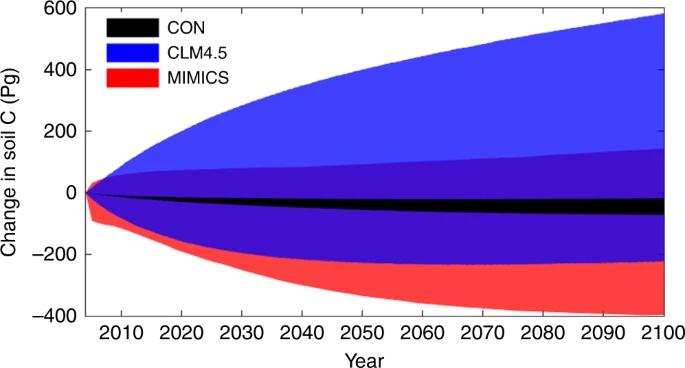
\includegraphics[width=0.6\textwidth,height=\textheight]{Zheng_et_al.png}
Shi, Zheng, Sean Crowell, Yiqi Luo, and Berrien Moore. ``Model
Structures Amplify Uncertainty in Predicted Soil Carbon Responses to
Climate Change.'' Nature Communications 9, no. 1 (June 4, 2018)
\end{frame}

\begin{frame}{Scary: linear algebra for linear models}
\protect\hypertarget{scary-linear-algebra-for-linear-models}{}
Compartmental models can be expressed within a generic linear algebra
(matrix) notation \[
\frac{dC_{(t)}}{dt}=I_{(t)} + A_{(t)} \cdot C_{(t)}
\] For example the ICBM model (assuming constant average inputs),
written explicitly, is: \[
 \frac{dC_{(t)}}{dt}=\begin{bmatrix} I\\  0\\  \end{bmatrix} +
  \xi \cdot
    \begin{bmatrix} -k_y & \epsilon \\ 0 & -k_o  \end{bmatrix} \cdot
    \begin{bmatrix} Y \\ O \end{bmatrix}
\] This notation allows us to generalize the main differences between
model structures:

\begin{longtable}[]{@{}
  >{\raggedright\arraybackslash}p{(\columnwidth - 4\tabcolsep) * \real{0.1158}}
  >{\raggedright\arraybackslash}p{(\columnwidth - 4\tabcolsep) * \real{0.4211}}
  >{\raggedright\arraybackslash}p{(\columnwidth - 4\tabcolsep) * \real{0.4632}}@{}}
\toprule()
\begin{minipage}[b]{\linewidth}\raggedright
\end{minipage} & \begin{minipage}[b]{\linewidth}\raggedright
Autonomous
\end{minipage} & \begin{minipage}[b]{\linewidth}\raggedright
Non-autonomous
\end{minipage} \\
\midrule()
\endhead
Linear & \(I+\xi \cdot A \cdot C_{(t)}\) &
\(I+\xi_{(t)} \cdot A \cdot C_{(t)}\) \\
Non-linear & \(I+\xi \cdot A (C_{(t)}) \cdot C_{(t)}\) &
\(I+\xi (t) \cdot A (C_{(t)}) \cdot C_{(t)}\) \\
\bottomrule()
\end{longtable}

(it brings also the pretty neat advantage of an easy nalytical steady
state for anything linear\ldots)
\end{frame}

\end{document}
